\section{بخش اول: بارگذاری تصاویر و آستانه‌گذاری (Thresholding)}

\begin{stepbox}
\field{بخش صفر: بارگذاری و بررسی تصاویر}{
در این گام، تصاویر ورودی شامل حیوانات (اسب، ماهی و پلنگ سیاه) با استفاده از کتابخانه‌ی \lr{OpenCV} خوانده شدند. از آنجا که این کتابخانه تصاویر را به صورت پیش‌فرض در فضای رنگی \lr{BGR} بارگذاری می‌کند، برای نمایش صحیح آن‌ها را به فضای \lr{RGB} استاندارد تبدیل کردیم. همچنین با استفاده از متد \lr{dtype} بررسی شد که مقادیر ماتریس‌ها از نوع ۸ بیتی مثبت (\lr{uint8}) باشند.
}
\end{stepbox}

\begin{codebox}[بارگذاری تصاویر و بررسی ابعاد]
\begin{lstlisting}[language=Python]
import cv2
import matplotlib.pyplot as plt
Horse_bgr = cv2.imread("./Input_Images/Horse.jpg")
Horse_rgb = cv2.cvtColor(Horse_bgr, cv2.COLOR_BGR2RGB)
print("Horse Data Type:", Horse_rgb.dtype) # خروجی: uint8
\end{lstlisting}
\end{codebox}

\begin{stepbox}
\field{بخش یک: تولید کانال خاکستری و رسم هیستوگرام}{
برای بررسی امکان بخش‌بندی تصویر با استفاده از تکنیک آستانه‌گذاری، ابتدا حالت \lr{gray-scale} تصاویر تولید شد. سپس هر تصویر را به ۴ کانال مجزا (قرمز، سبز، آبی و خاکستری) تفکیک کرده و نمودار هیستوگرام (فراوانی شدت روشنایی) آن‌ها رسم گردید. هدف از این کار، یافتن کانالی بود که دارای دو قله‌ی مجزا باشد تا بتوان مرز مناسبی برای جداسازی حیوان از پس‌زمینه تعیین کرد.
}
\end{stepbox}

\begin{figure}[h!]
    \centering
    % مسیر تصویر را در صورت نیاز اصلاح کنید
    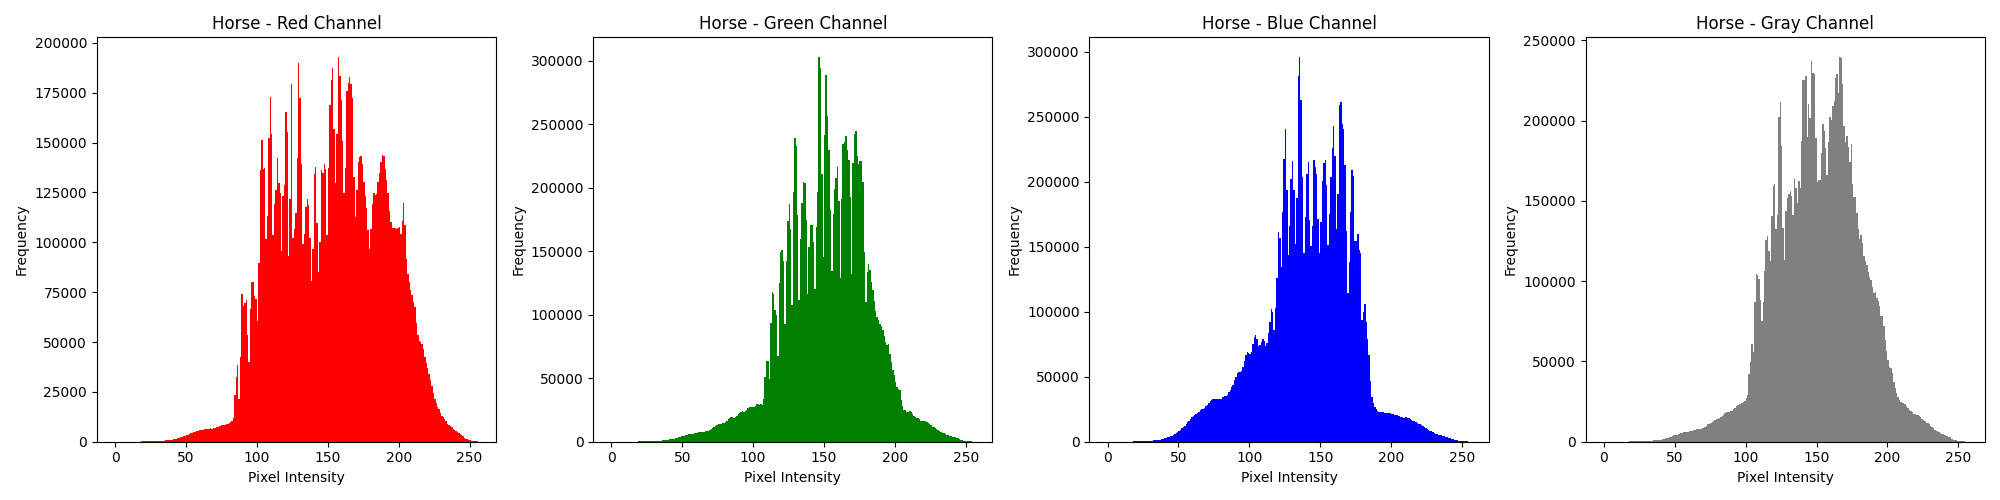
\includegraphics[width=\textwidth]{./images/Part_1/Horse_Histograms.png}
    \caption{رسم هیستوگرام ۴ کانال رنگی و خاکستری برای بررسی مقادیر پیکسل‌های تصویر اسب}
    \label{fig:horse_histograms}
\end{figure}

\begin{stepbox}
\field{پاسخ به سوال تمرین: تحلیل عملکرد روش آستانه‌گذاری}{
با اعمال مقادیر مختلف آستانه (به عنوان مثال اعداد ۱۰۰، ۱۵۰ و ۲۰۰) بر روی کانال خاکستری، تلاش شد تا سوژه از پس‌زمینه جدا شود؛ اما نتایج نشان داد که روش آستانه‌گذاری به کمک هیستوگرام برای تصاویر حیوانات در محیط زیست \textbf{عملکرد مناسبی ندارد}.

\textbf{علت:} روش آستانه‌گذاری سراسری (\lr{Global Thresholding}) تنها در تصاویری موفق است که تضاد (\lr{Contrast}) بالایی بین سوژه و پس‌زمینه وجود داشته باشد (تصاویر با هیستوگرام \lr{Bimodal}). در تصاویر واقعی طبیعت، شدت روشنایی و رنگ عناصر پس‌زمینه (مانند ابرها، گرد و خاک و گیاهان) با بافت بدن حیوانات هم‌پوشانی شدیدی دارد و هیچ "دره‌ی" عمیقی در هیستوگرام برای قرار دادن خط آستانه وجود ندارد.
}
\end{stepbox}

\begin{figure}[h!]
    \centering
    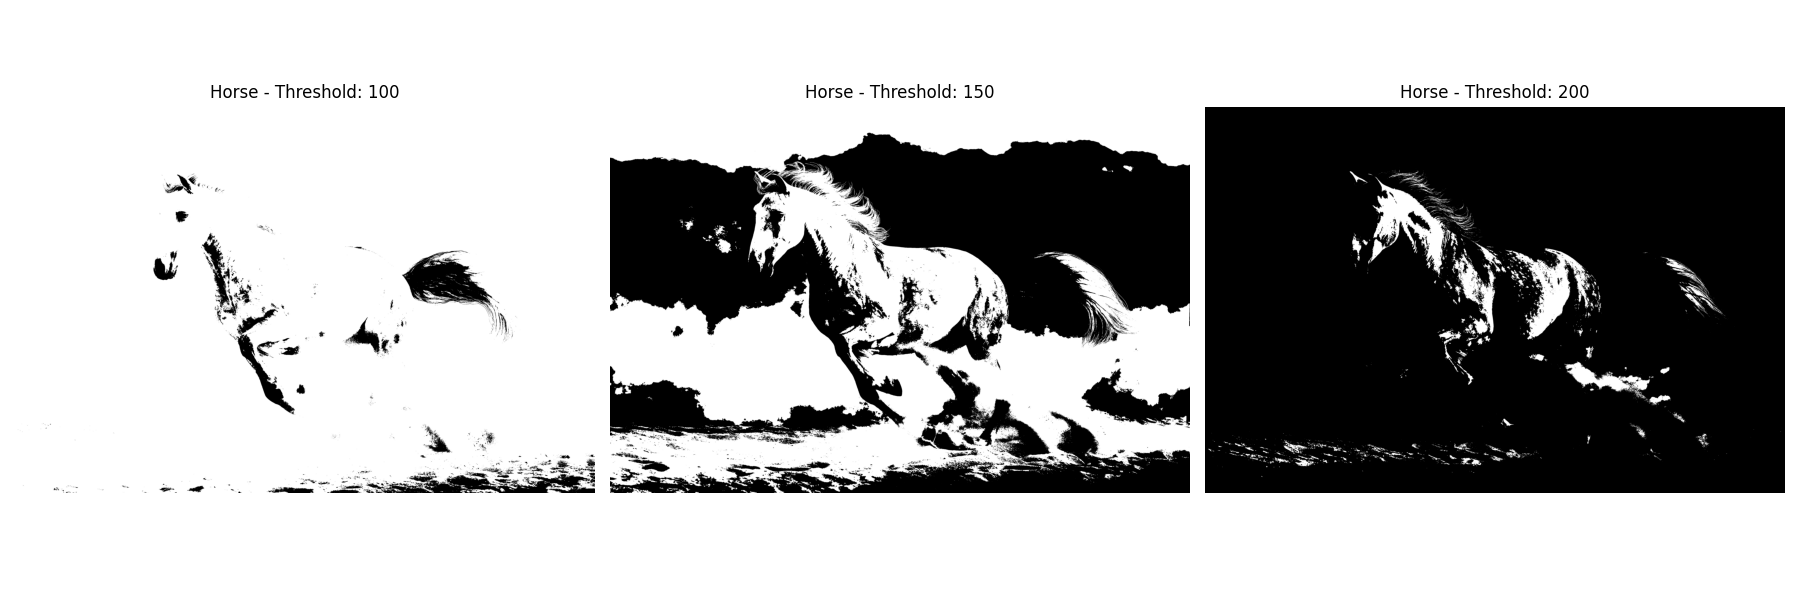
\includegraphics[width=\textwidth]{./images/Part_1/Horse_Thresholds_Comparison.png}
    \caption{مقایسه‌ی اعمال مقادیر مختلف آستانه روی تصویر اسب؛ هم‌پوشانی مقادیر باعث عدم تفکیک صحیح می‌شود.}
    \label{fig:horse_threshold_comparison}
\end{figure}

\begin{tipbox}[بهبود فرآیند]
برای اجرای خودکار این فرآیند روی تمامی تصاویر، یک تابع سفارشی پایتون به نام \lr{\texttt{apply\_threshold}} نوشته شد تا لیستی از مقادیر آستانه را دریافت کرده و نتایج را در قالب یک \lr{Subplot} در کنار یکدیگر برای مقایسه بصری ترسیم کند.
\end{tipbox}